\documentclass[10pt,a4paper]{article}
\usepackage[utf8]{inputenc}
\usepackage{amsmath}
\usepackage{amsfonts}
\usepackage{amssymb}
\usepackage{makeidx}
\usepackage{graphicx}
\usepackage{xcolor}
\usepackage{listings}
\usepackage{caption}
\DeclareCaptionFont{white}{\color{white}}
\DeclareCaptionFormat{listing}{%
  \parbox{\textwidth}{\colorbox{gray}{\parbox{\textwidth}{#1#2#3}}\vskip-4pt}}
\captionsetup[lstlisting]{format=listing,labelfont=white,textfont=white}
\lstset{frame=lrb,xleftmargin=\fboxsep,xrightmargin=-\fboxsep}
\author{Shravan Kumar P}
\title{Assignment2}

\begin{document}
\maketitle
Here I reported my assignment work with respect to the questions given. All the code is implemented using   python in Jupyter Notebook. 

\tableofcontents
\section{Problem 1}
\subsection{Perceptron Algorithm:}
1.Use the data given in Table 1. Starting with w = [0 0] T and b = 0,apply your program to learn a linear classifier to separate classes C 1 and C 2 . Plot the data points for C 1 and C 2 . Plot the final classifier learnt at the convergence. Note the number of iterations required for convergence.

The algorithm implemented as taught in class(referring R.Duda Text Book). 
The Class1 and class2 data has 10 instances and 2 features. similarly for C2and C3. 
I have agumented the $10\times2$ matrix with all ones in the beginning to make it a $10\times3$ matrix.
and added bias(threshold) term into the weight vector. Therefore my new weight vector is of size $3\times1$ istead $2\times1$. 

Along with I have multiplied Class2 samples with -1, so that now I can decide the samples as misclassified if they are less than zero. 

If the particular sample get misclassified then we do weight update using gradient descent method.

\graphicspath{ {/images/} }
\begin{figure}[h!]
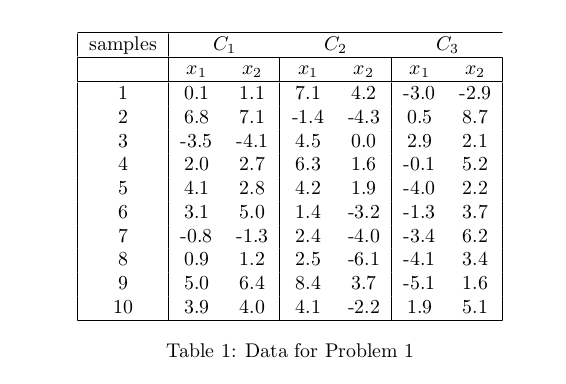
\includegraphics[scale=0.5]{images/problem1T.png}
  \caption{Table1}
  \label{fig:dataT1}
\end{figure}
\vfill
%%%%%%%%%%%%%%%%%%%%%%%%%%%%%%%%%%%%%%%%%%%%%%%%%%%%%%%%%%%%%%%%%%%%%%%%%%%%%%%%%%%%%%%%%

\lstset{% general command to set parameter(s)
basicstyle=\small, % print whole listing small
identifierstyle=, % nothing happens
stringstyle=\ttfamily, % typewriter type for strings
showstringspaces=false} % no special string spaces

\lstset{language=Python}          % Set your language (you can change the language for each code-block optionally)

\begin{lstlisting}[label=perceptron,caption=Perceptron]  % Start your code-block

def percp(train, weights, nb_epoch=1):
    w = weights
    X = train
    for epoc in range(nb_epoch):
        print("*************************")
        print("Epoch {}".format(epoc))
        print("*************************")
        print(" ")
        print("current weights {}".format(w))
        print(" ")
        for i in range(len(X)):
            print("iteration{} on X{}".format(i,i))
            y = np.dot(X[i],w)
            count = 0
            if y<=0:
                print("xxxxxxx")
                print("Misclassified sample x{}".format(i))
                print("-------")
                w = w+X[i]
                print("-------")
                print("updated weight w = {}".format(w))
                print(":) :) :) ")
#                 count +=1
#                 print("inside {}".format(count))
#             print("outside {}".format(count))
        print(" ")           
        print("Finally the best weight vector is {} at iteration {}".format(w,epoc))
        print(" ")
    print(w)
    return w
    
\end{lstlisting}
\vfill

\textbf{Linear Classfier that discrimnate the two classes C1, C2 using the above solution vector}
At Iteration 7, the algorithm find the solution vector as w = [ 13. -10.2 11.3]

\graphicspath{ {/images/} }
\begin{figure}[h!]
\centering
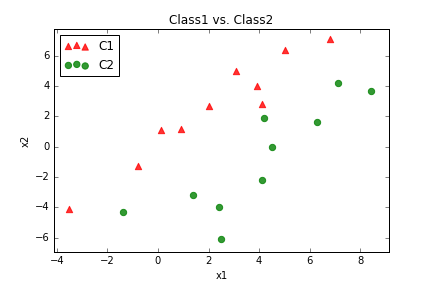
\includegraphics[scale=0.5]{images/P1_C1C2.png}
  \caption{Class1 vs. Class2}
  \label{fig:p11}
\end{figure}

\graphicspath{ {/images/} }
\begin{figure}[h!]
\centering
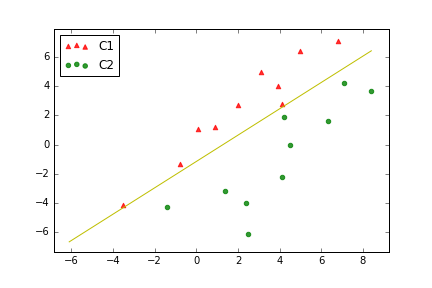
\includegraphics[scale=0.5]{images/P1_C12_classified.png}
  \caption{Linear classification}
  \label{fig:p12}
\end{figure}

\textbf{Linear Classfier that discrimnate the two classes C2, C3 using the above solution vector}
At Iteration 4, the algorithm find the solution vector as w = [-5. 5.5 -6.4]

\graphicspath{ {/images/} }
\begin{figure}[h!]
\centering
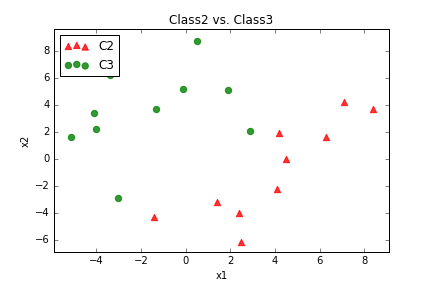
\includegraphics[scale=0.5]{images/P1_C2C3.png}
  \caption{Class2 vs. Class3}
  \label{fig:p13}
\end{figure}

\graphicspath{ {/images/} }

\begin{figure}[h!]
\centering
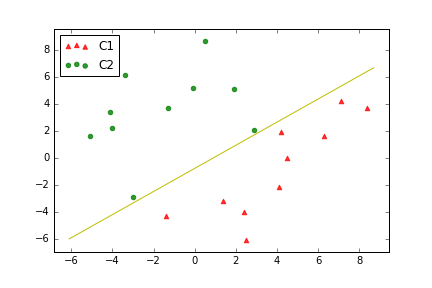
\includegraphics[scale=0.5]{images/P1_C23_classified.png}
  \caption{Linear Classification }
  \label{fig:p14}
\end{figure}

From the figure above, the features of C1, C2 (figure (\ref{fig:p11}) ) are closely coupled as compared to the features of C2,C3 (figure(\ref{fig:p13})).
Hence finding the optimally best solution vector for (C1,C2) takes more number of iterations thatn finding an optimally best solution for (C2,C3), 7, 4 number of iterations respectively.

\vfill
%%%%%%%%%%%%%%%%%%%%%%%%%%%%%%%%%%%%%%%%%%%%%%%%%%%%%%%%%%%%%%%%%%%%%%%%%%%%%%%%%%%%%%%%%

\section{Problem 2}
\subsection*{voted-perceptron algorithm}
%%%%%%%%%%%%%%%%%%%%%%%%%%%%%%%%%%%%%%%%%%%%%%%%%%%%%%%%%%%%%%%%%%%%%%%%%%%%%%%%%%%%%%%%%

\lstset{% general command to set parameter(s)
basicstyle=\small, % print whole listing small
identifierstyle=, % nothing happens
stringstyle=\ttfamily, % typewriter type for strings
showstringspaces=false} % no special string spaces

\lstset{language=Python}          % Set your language (you can change the language for each code-block optionally)

\begin{lstlisting}[label=vperceptron,caption=Voted-Perceptron]  % Start your code-block

def vpercp(X, Y, nb_epoch=1,kfold=10):
    w1 = np.zeros(features.shape[1])
    c1 = 1
    v1 = []
    p1 = []    
    for epoch in range(nb_epoch):
        for x,y in zip(X,Y):
            u = np.inner(x,w1)
            if y*u<=0:
                v1.append(w1)
                p1.append(c1)
                w1 = w1+y*x
                c1 = 1
            else:
                c1 =c1+1
    return v1,p1
\end{lstlisting}
\vfill
%%%%%%%%%%%%%%%%%%%%%%%%%%%%%%%%%%%%%%%%%%%%%%%%%%%%%%%%%%%%%%%%%%%%%%%%%%%%%%%%%%%%%%%%%
\subsection*{perceptron algorithm}
%%%%%%%%%%%%%%%%%%%%%%%%%%%%%%%%%%%%%%%%%%%%%%%%%%%%%%%%%%%%%%%%%%%%%%%%%%%%%%%%%%%%%%%%%

\lstset{% general command to set parameter(s)
basicstyle=\small, % print whole listing small
identifierstyle=, % nothing happens
stringstyle=\ttfamily, % typewriter type for strings
showstringspaces=false} % no special string spaces

\lstset{language=Python}          % Set your language (you can change the language for each code-block optionally)

\begin{lstlisting}[label=percep,caption=Perceptron]  % Start your code-block

def percp(X, Y, nb_epoch=1):
    w = np.zeros(X.shape[1])
    for epoch in range(nb_epoch):
        for x,y in zip(X,Y):
            if y*np.dot(x,w)<=0:
                w = w+y*x
    return w
\end{lstlisting}
\vfill
%%%%%%%%%%%%%%%%%%%%%%%%%%%%%%%%%%%%%%%%%%%%%%%%%%%%%%%%%%%%%%%%%%%%%%%%%%%%%%%%%%%%%%%%%

\subsection{breast-cancer-wisconsin}
\graphicspath{ {/images/} }
\begin{figure}[!h]
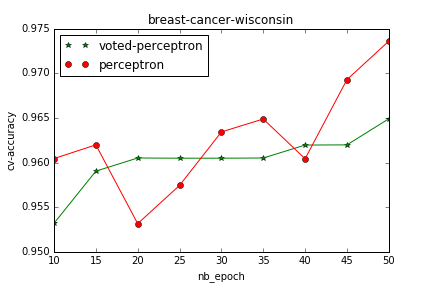
\includegraphics[scale=0.75]{images/bcresult.png}	
\end{figure}
\textbf{Remove the rows corresponding to missing values in Breast Cancer Dataset}
%%%%%%%%%%%%%%%%%%%%%%%%%%%%%%%%%%%%%%%%%%%%%%%%%%%%%%%%%%%%%%%%%%%%%%%%%%%%%%%%%%%%%%%%%

\lstset{% general command to set parameter(s)
basicstyle=\small, % print whole listing small
identifierstyle=, % nothing happens
stringstyle=\ttfamily, % typewriter type for strings
showstringspaces=false} % no special string spaces

\lstset{language=Python}          % Set your language (you can change the language for each code-block optionally)

\begin{lstlisting} [label=remove_unknwn,caption=To remove missing values] % Start your code-block
df = pd.read_csv('../datasets/breast-cancer-wisconsin.csv', header=None)
df = df[(df[6]!='?')].astype('float')
del df[0]
n = 1
\end{lstlisting}
%%%%%%%%%%%%%%%%%%%%%%%%%%%%%%%%%%%%%%%%%%%%%%%%%%%%%%%%%%%%%%%%%%%%%%%%%%%%%%%%%%%%%%%%%



\subsection{ionosphere}
\graphicspath{ {/images/} }
\begin{figure}[!h]
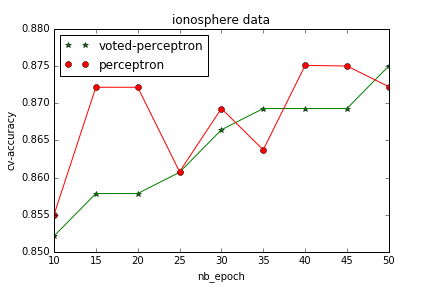
\includegraphics[scale=0.75]{images/ionosphere_result.png}	
\end{figure}
\clearpage


\section{Problem 3}
Figure \ref{fig:C12T1}
\graphicspath{ {/images/} }
\begin{figure}[!h]
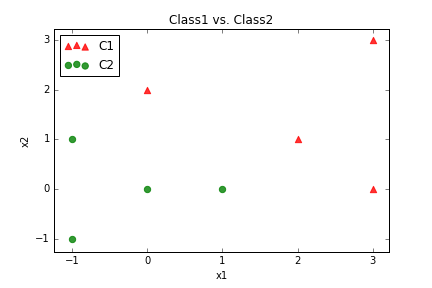
\includegraphics[scale=0.75]{images/C1vsC2_Table1.png}
  \caption{C1vsC2-Table1}
  \label{fig:C12T1}
\end{figure}

\graphicspath{ {/images/} }
\begin{figure}[!h]
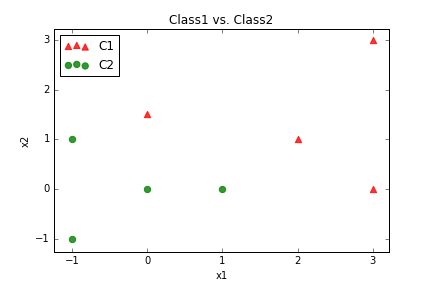
\includegraphics[scale=0.75]{images/C3vsC4_Table2.png}	
  \caption{C1vsC2-Table2}
  \label{fig:C34T2}
\end{figure}

\subsection{Least Squares Method}
\graphicspath{ {/images/} }
\begin{figure}[!h]
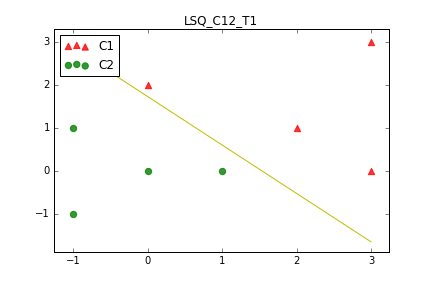
\includegraphics[scale=0.75]{images/LSQ_C12_T1.png}	
  \caption{LSQ-C1vsC2-Table1}
  \label{fig:LC12T1}
\end{figure}

\graphicspath{ {/images/} }
\begin{figure}[!h]
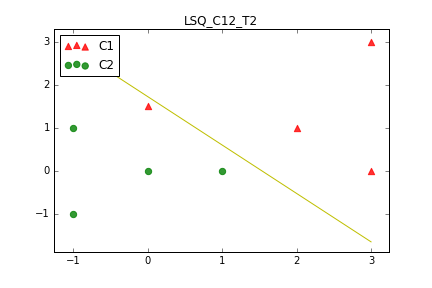
\includegraphics[scale=0.75]{images/LSQ_C12_T2.png}	
  \caption{LSQ-C1vsC2-Table2}
  \label{fig:LC12T2}
\end{figure}
%%%%%%%%%%%%%%%%%%%%%%%%%%%%%%%%%%%%%%%%%%%%%%%%%%%%%%%%%%%%%%%%%%%%%%%%%%%%%%%%%%%%%%%%%

\lstset{% general command to set parameter(s)
basicstyle=\small, % print whole listing small
identifierstyle=, % nothing happens
stringstyle=\ttfamily, % typewriter type for strings
showstringspaces=false} % no special string spaces

\lstset{language=Python}          % Set your language (you can change the language for each code-block optionally)

\begin{lstlisting} [label=lsq,caption=Least Square Method] % Start your code-block

def lsq(X12,b=None):
    b = np.ones(len(X12))
    w = np.dot(np.linalg.pinv(X12),b)
    return w  


\end{lstlisting}
\vfill
%%%%%%%%%%%%%%%%%%%%%%%%%%%%%%%%%%%%%%%%%%%%%%%%%%%%%%%%%%%%%%%%%%%%%%%%%%%%%%%%%%%%%%%%%
\subsection{Fisher's LDA}

%%%%%%%%%%%%%%%%%%%%%%%%%%%%%%%%%%%%%%%%%%%%%%%%%%%%%%%%%%%%%%%%%%%%%%%%%%%%%%%%%%%%%%%%%

\lstset{% general command to set parameter(s)
basicstyle=\small, % print whole listing small
identifierstyle=, % nothing happens
stringstyle=\ttfamily, % typewriter type for strings
showstringspaces=false} % no special string spaces

\lstset{language=Python}          % Set your language (you can change the language for each code-block optionally)

\begin{lstlisting}[label=flda,caption=Fisher's Linear Discriminant]  % Start your code-block

def flda(c1,c2,p=False):
    u1 = np.mean(c1, axis=0)
    u2 = np.mean(c2, axis=0)
    S1 = (len(c1) -1)*np.cov(c1.T)
    S2 = (len(c2 -1))*np.cov(c2.T)
    Sw = np.add(S1,S2)
    iSw = np.linalg.pinv(Sw)
    v = np.dot(iSw,(u1-u2))
    if p:
        v1 = np.c_[v, v]
        plotv(v1)
    return v
    
\end{lstlisting}
\vfill
\graphicspath{ {/images/} }
\begin{figure}[!h]
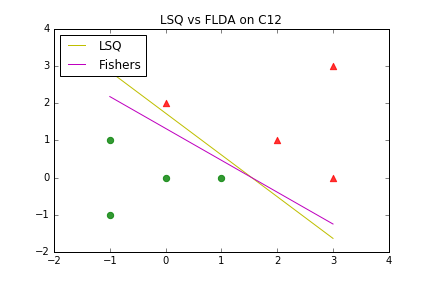
\includegraphics[scale=0.75]{images/LsqvsFLDA_C12.png}	
  \caption{LSQ-FLDA-C1vsC2-Table1}
  \label{fig:C34T2}
\end{figure}

\graphicspath{ {/images/} }
\begin{figure}[!h]
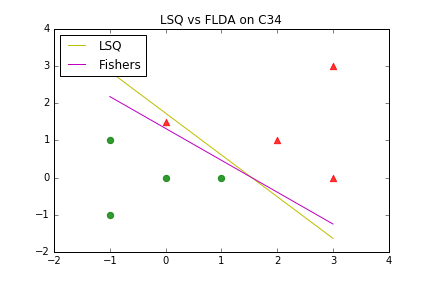
\includegraphics[scale=0.75]{images/LsqvsFLDA_C34.png}	
  \caption{LSQ-FLDA-C3vsC4-Table2}
  \label{fig:C34T2}
\end{figure}
%%%%%%%%%%%%%%%%%%%%%%%%%%%%%%%%%%%%%%%%%%%%%%%%%%%%%%%%%%%%%%%%%%%%%%%%%%%%%%%%%%%%%%%%%
\section{Problem 4}
\subsection{Relation between Least Squares and
Fisher's linear discriminant}

\graphicspath{ {/images/} }
\begin{figure}[!h]
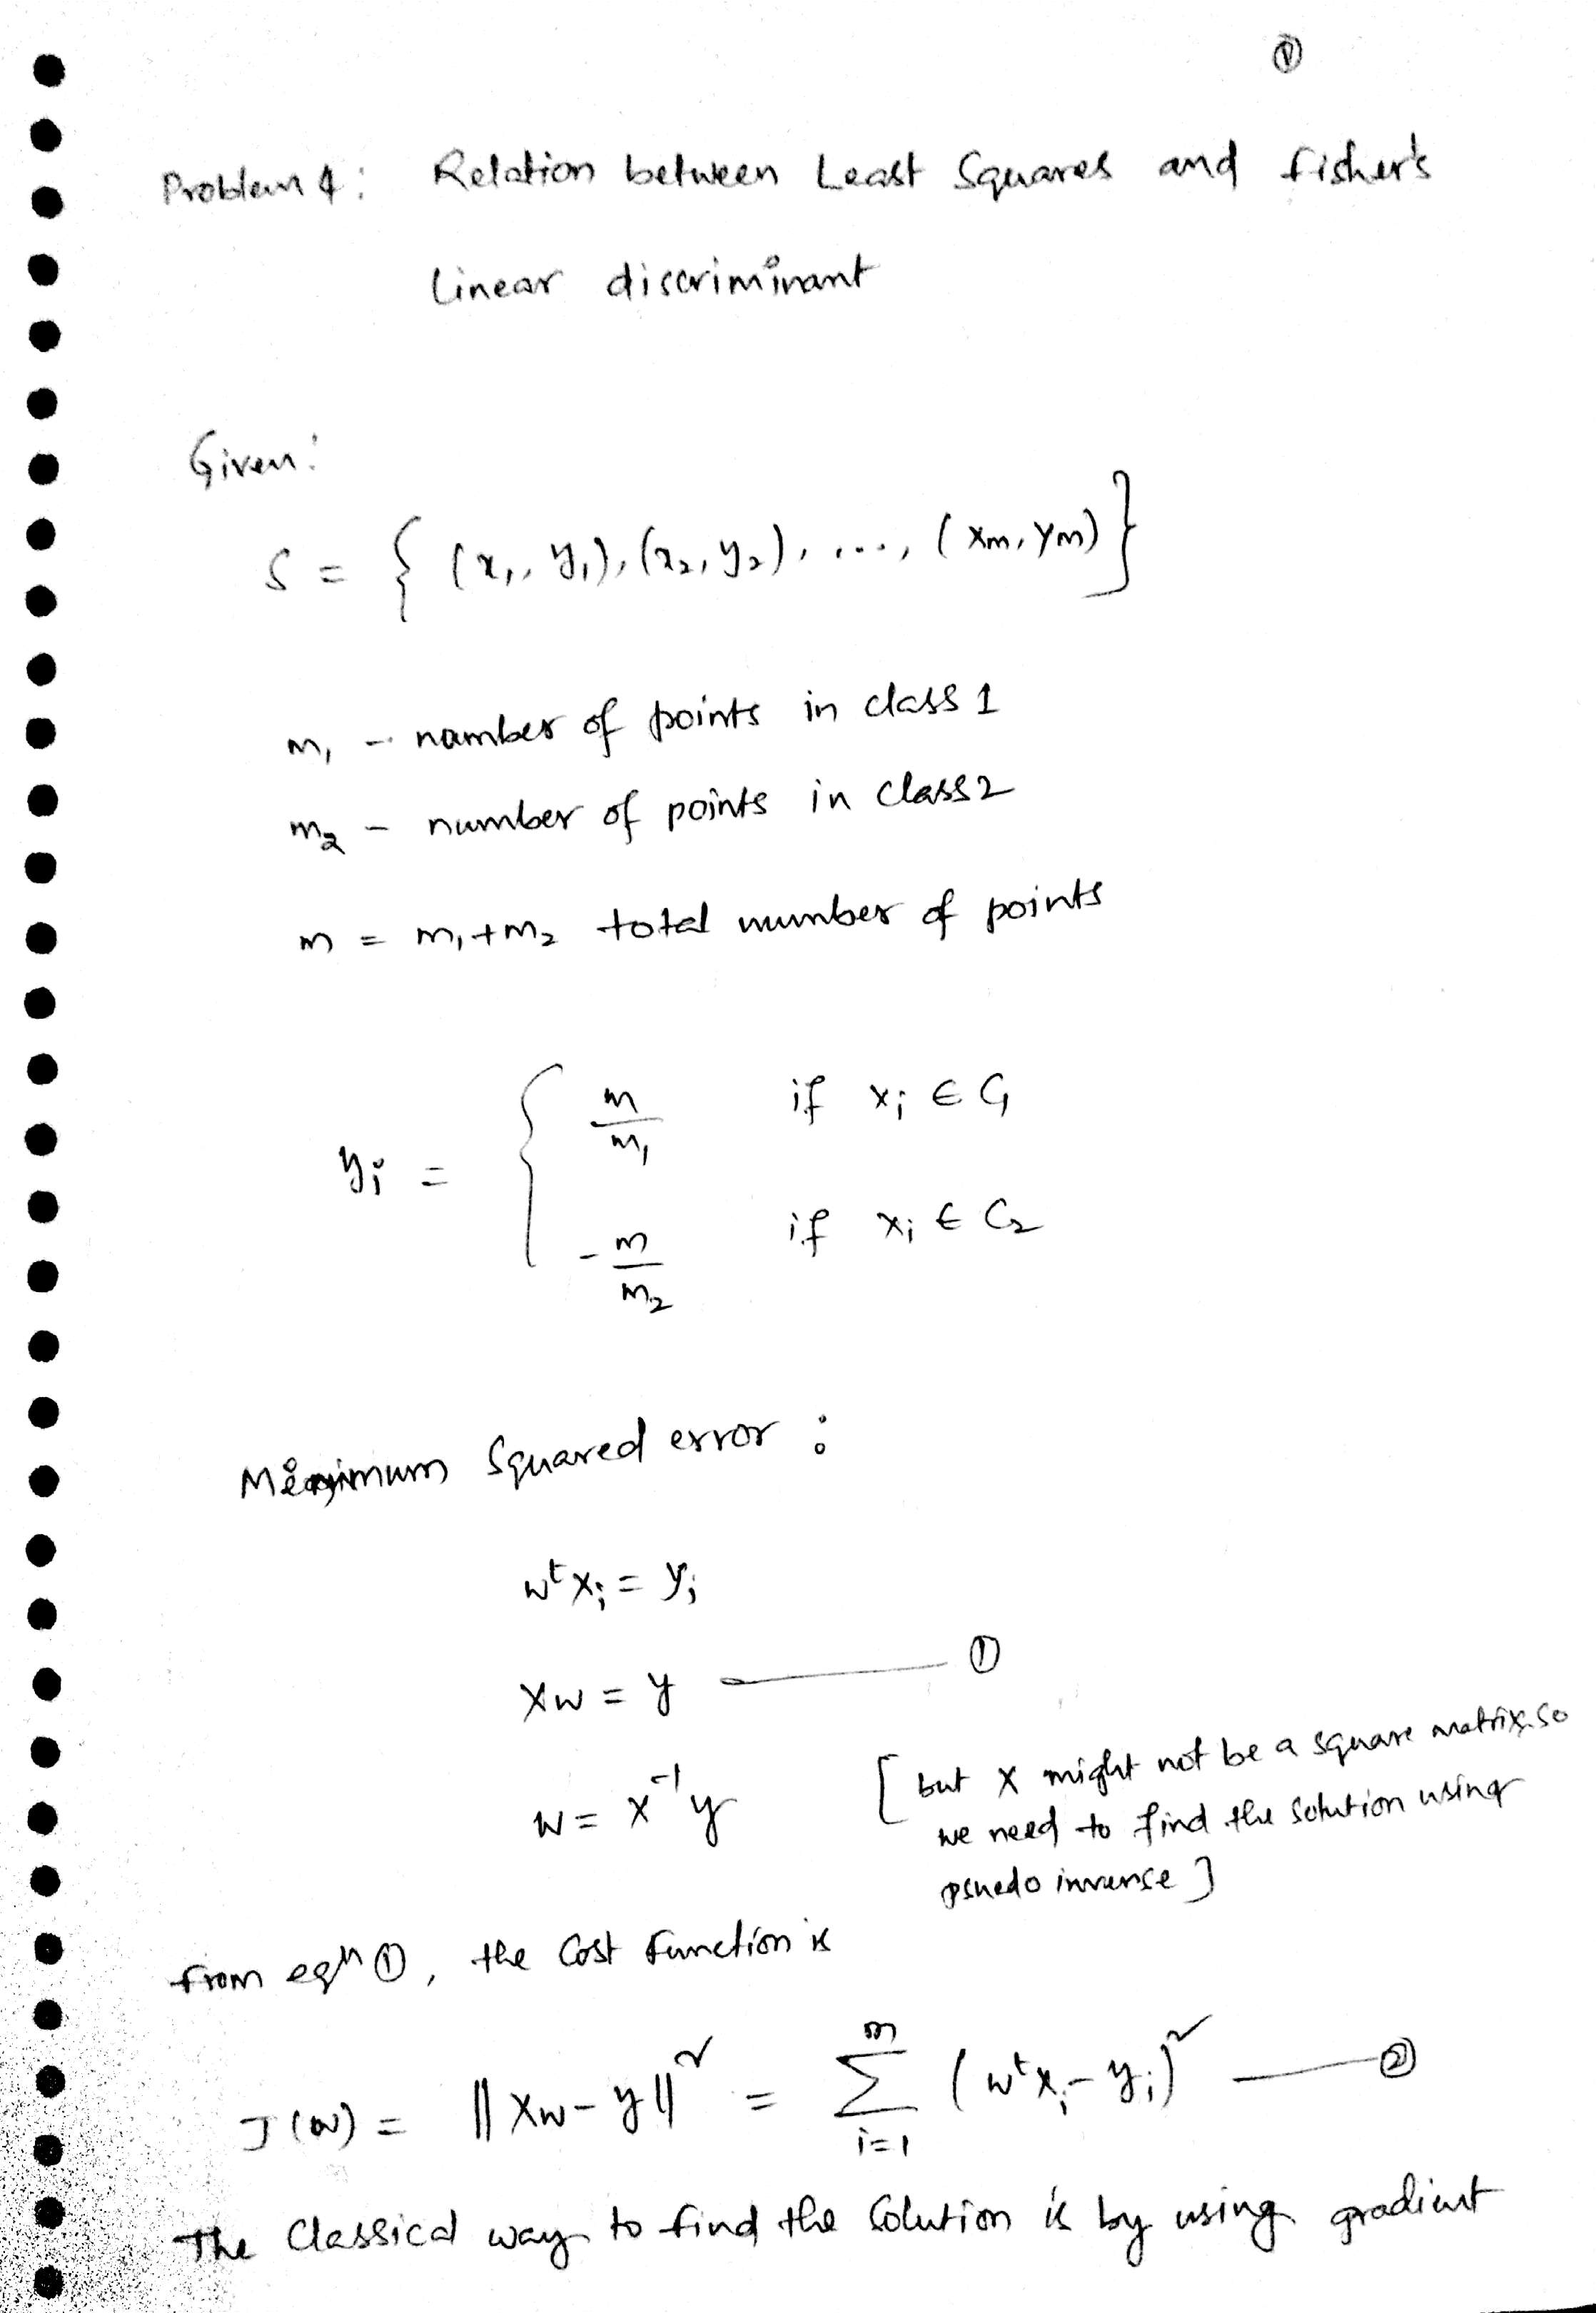
\includegraphics[scale=0.03]{images/p4A2_1.jpg}	
  \caption{p1}
  \label{fig:C34T2}
\end{figure}
\graphicspath{ {/images/} }
\begin{figure}[!h]
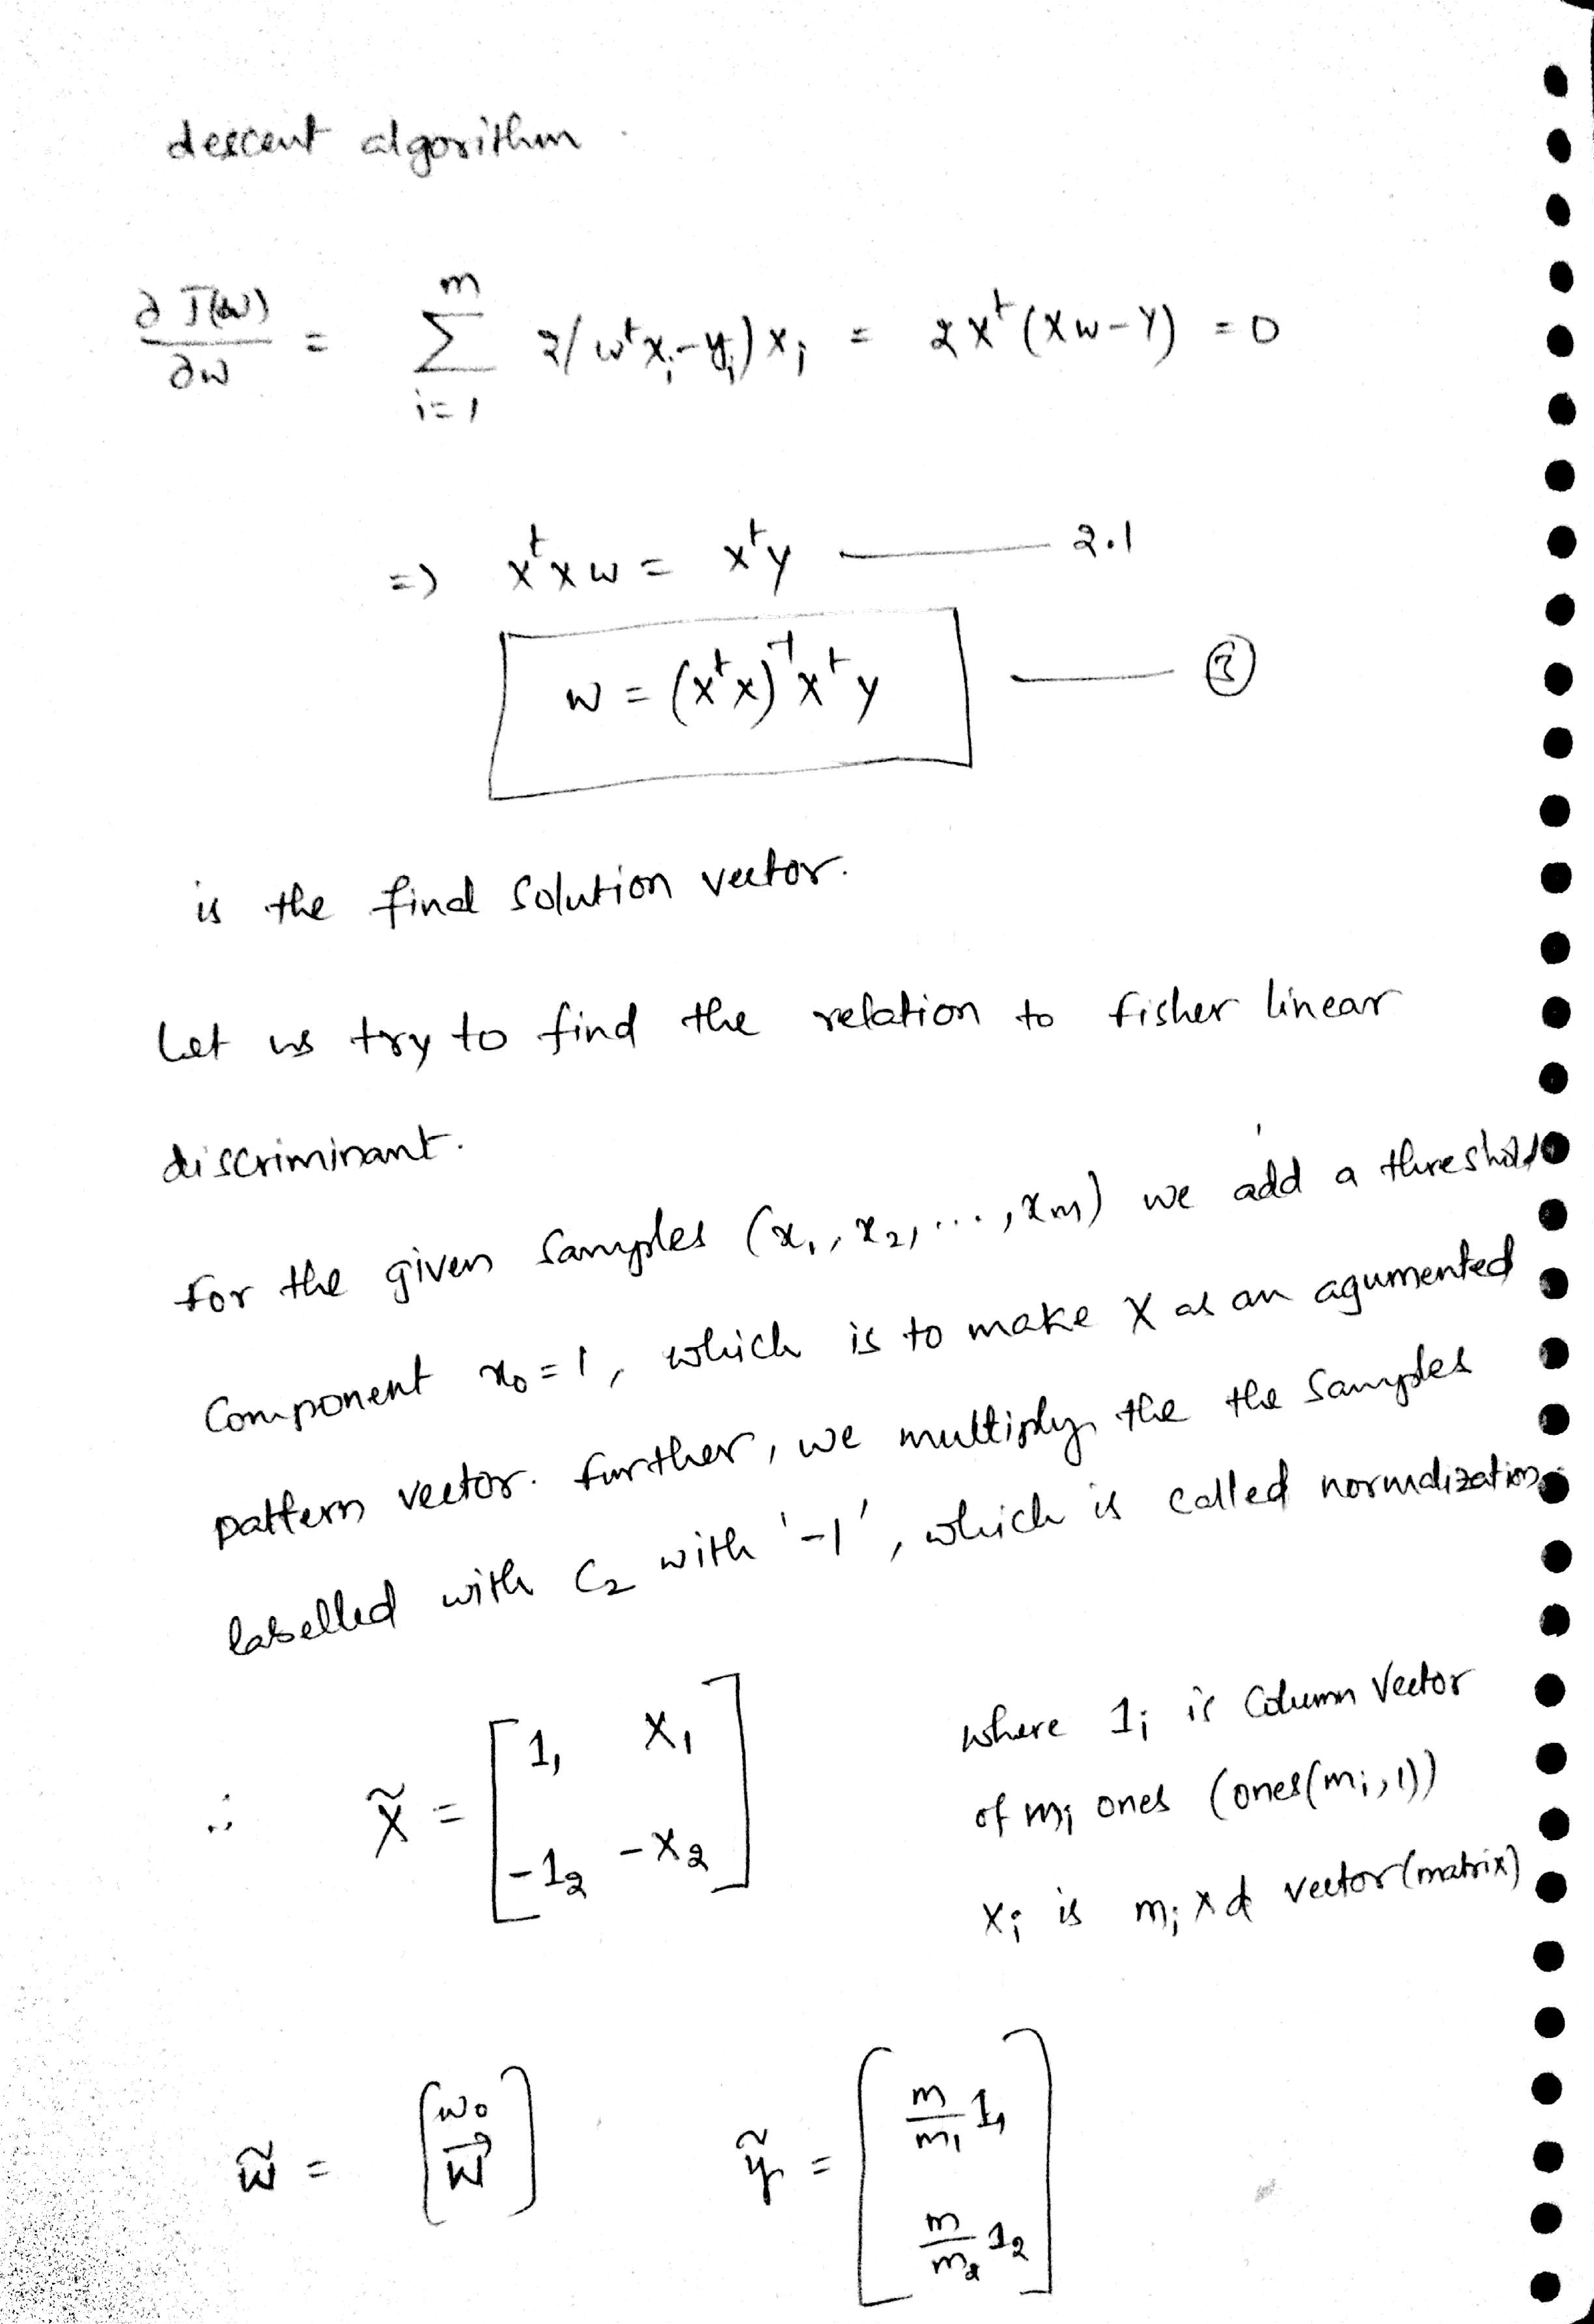
\includegraphics[scale=0.03]{images/p4A2_2.jpg}	
  \caption{p2}
  \label{fig:C34T2}
\end{figure}
\graphicspath{ {/images/} }
\begin{figure}[!h]
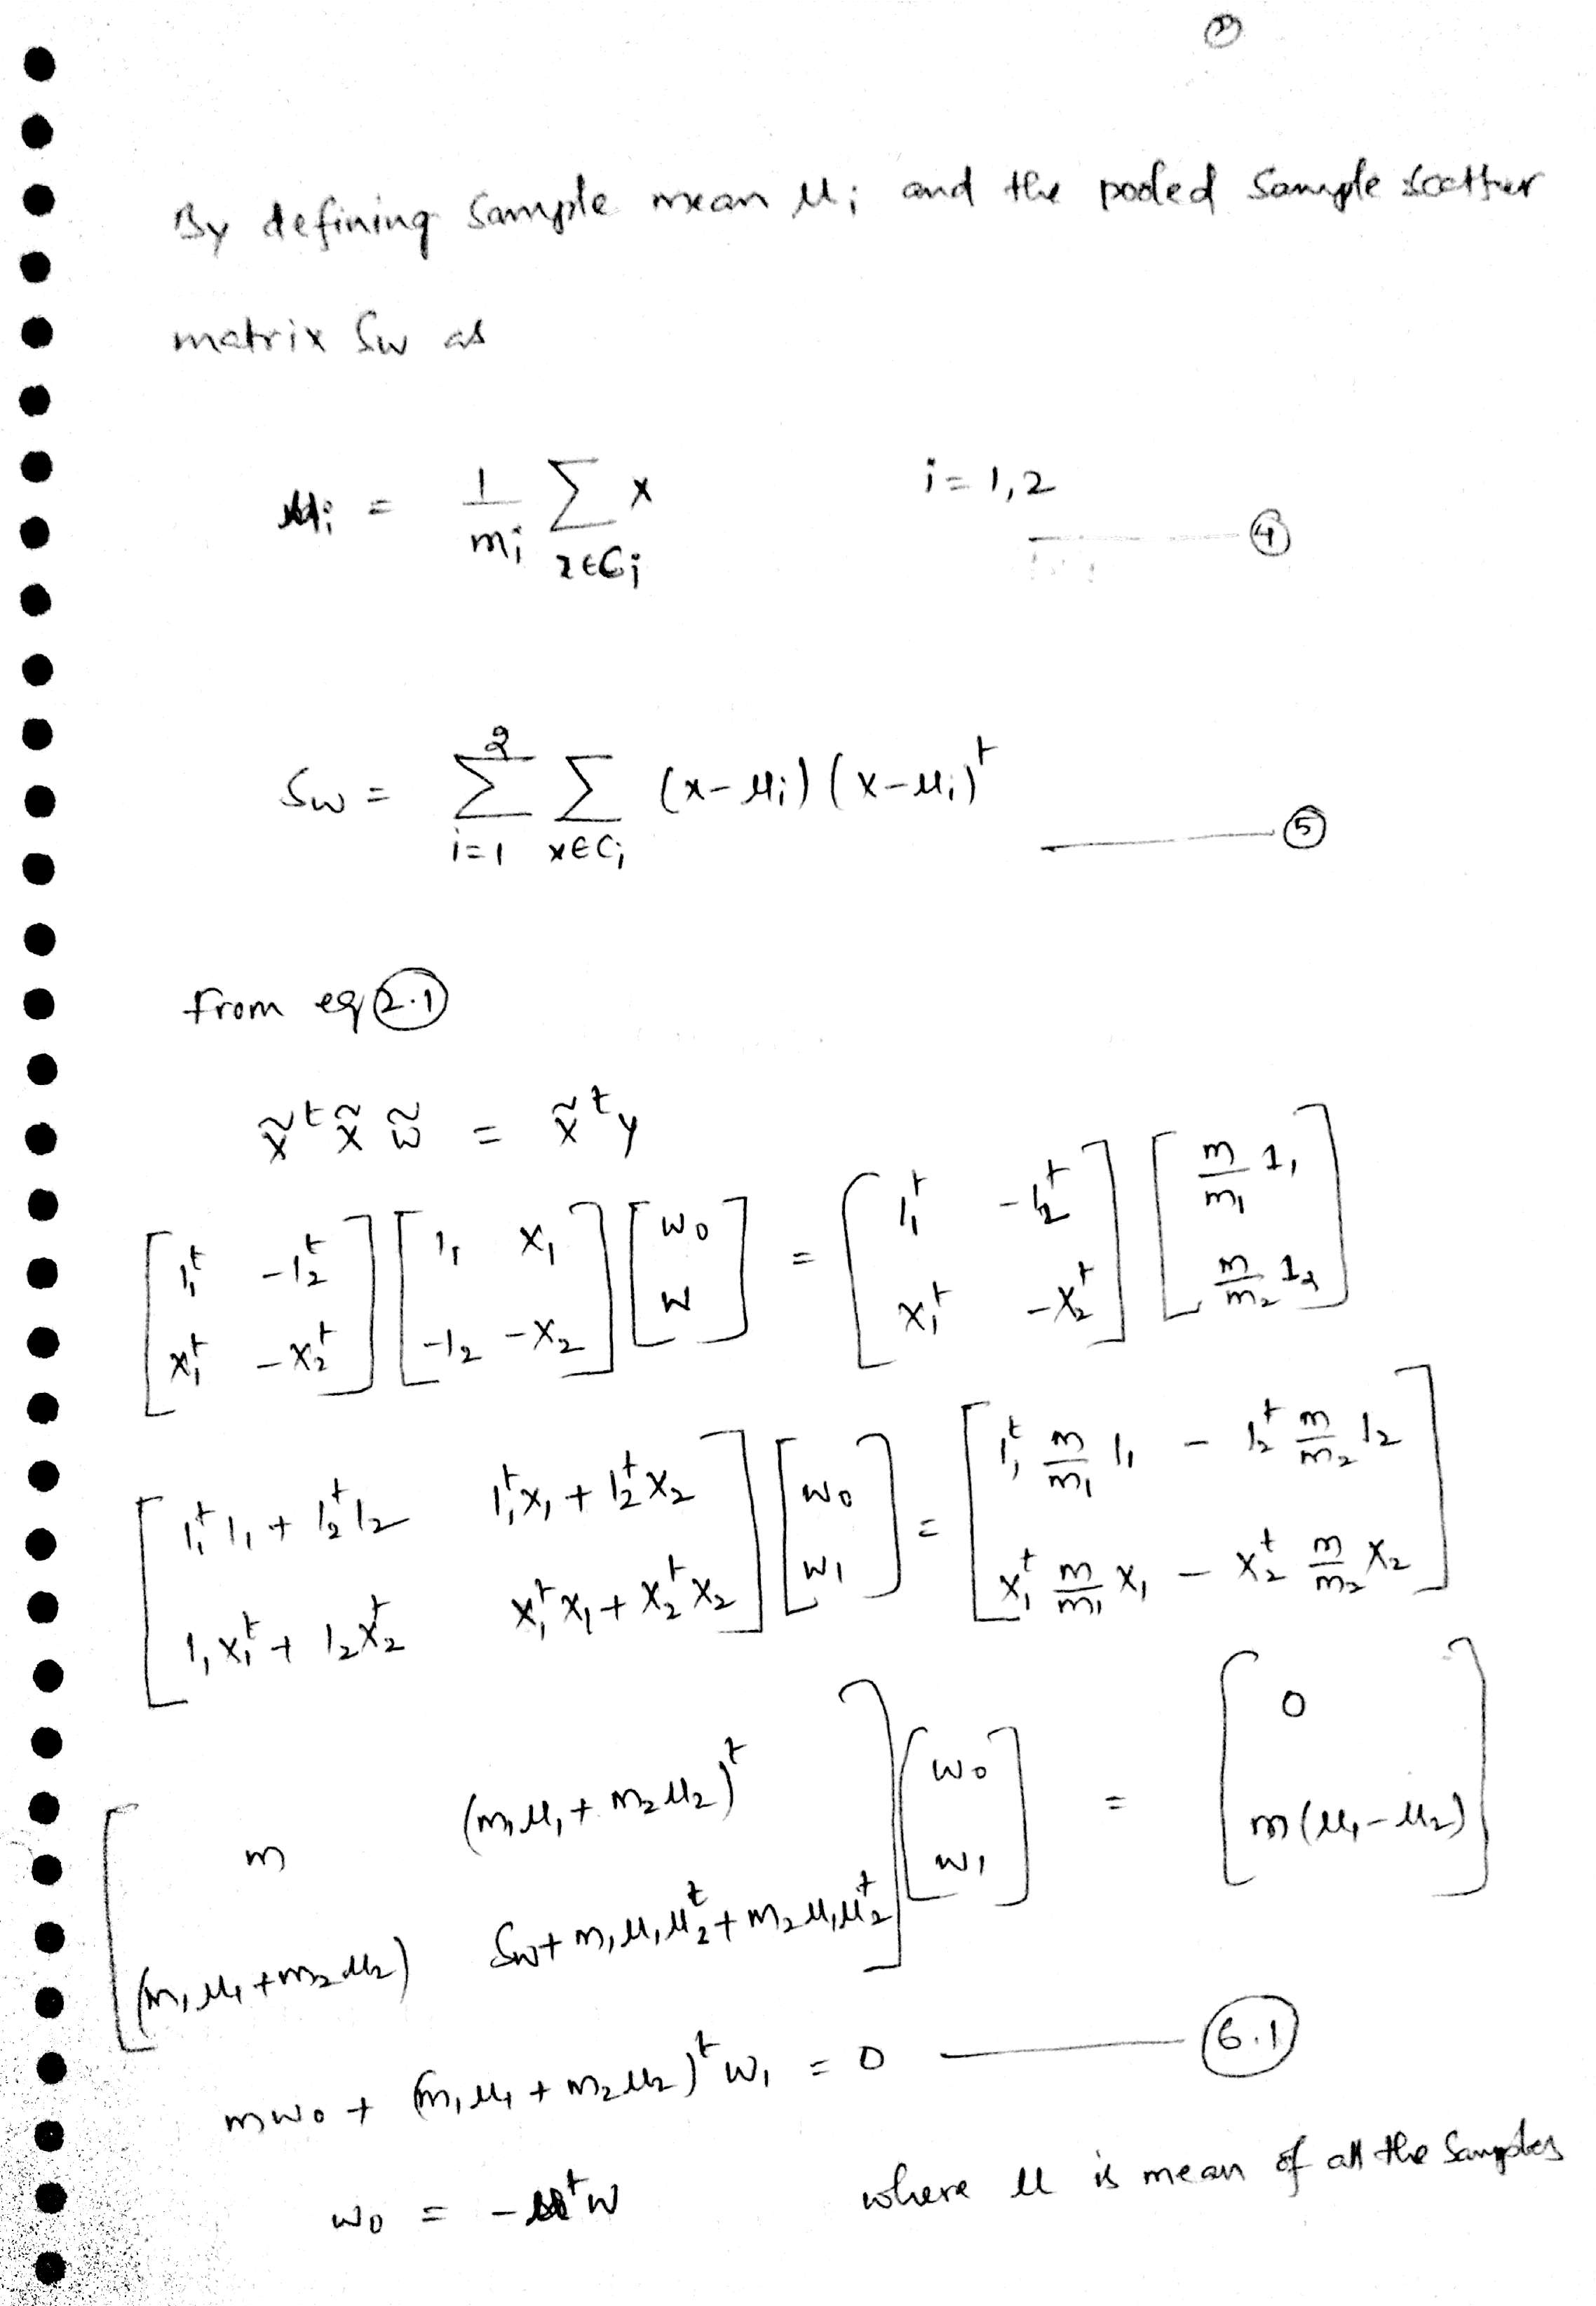
\includegraphics[scale=0.03]{images/p4A2_3.jpg}	
  \caption{p3}
  \label{fig:C34T2}
\end{figure}
\graphicspath{ {/images/} }
\begin{figure}[!h]
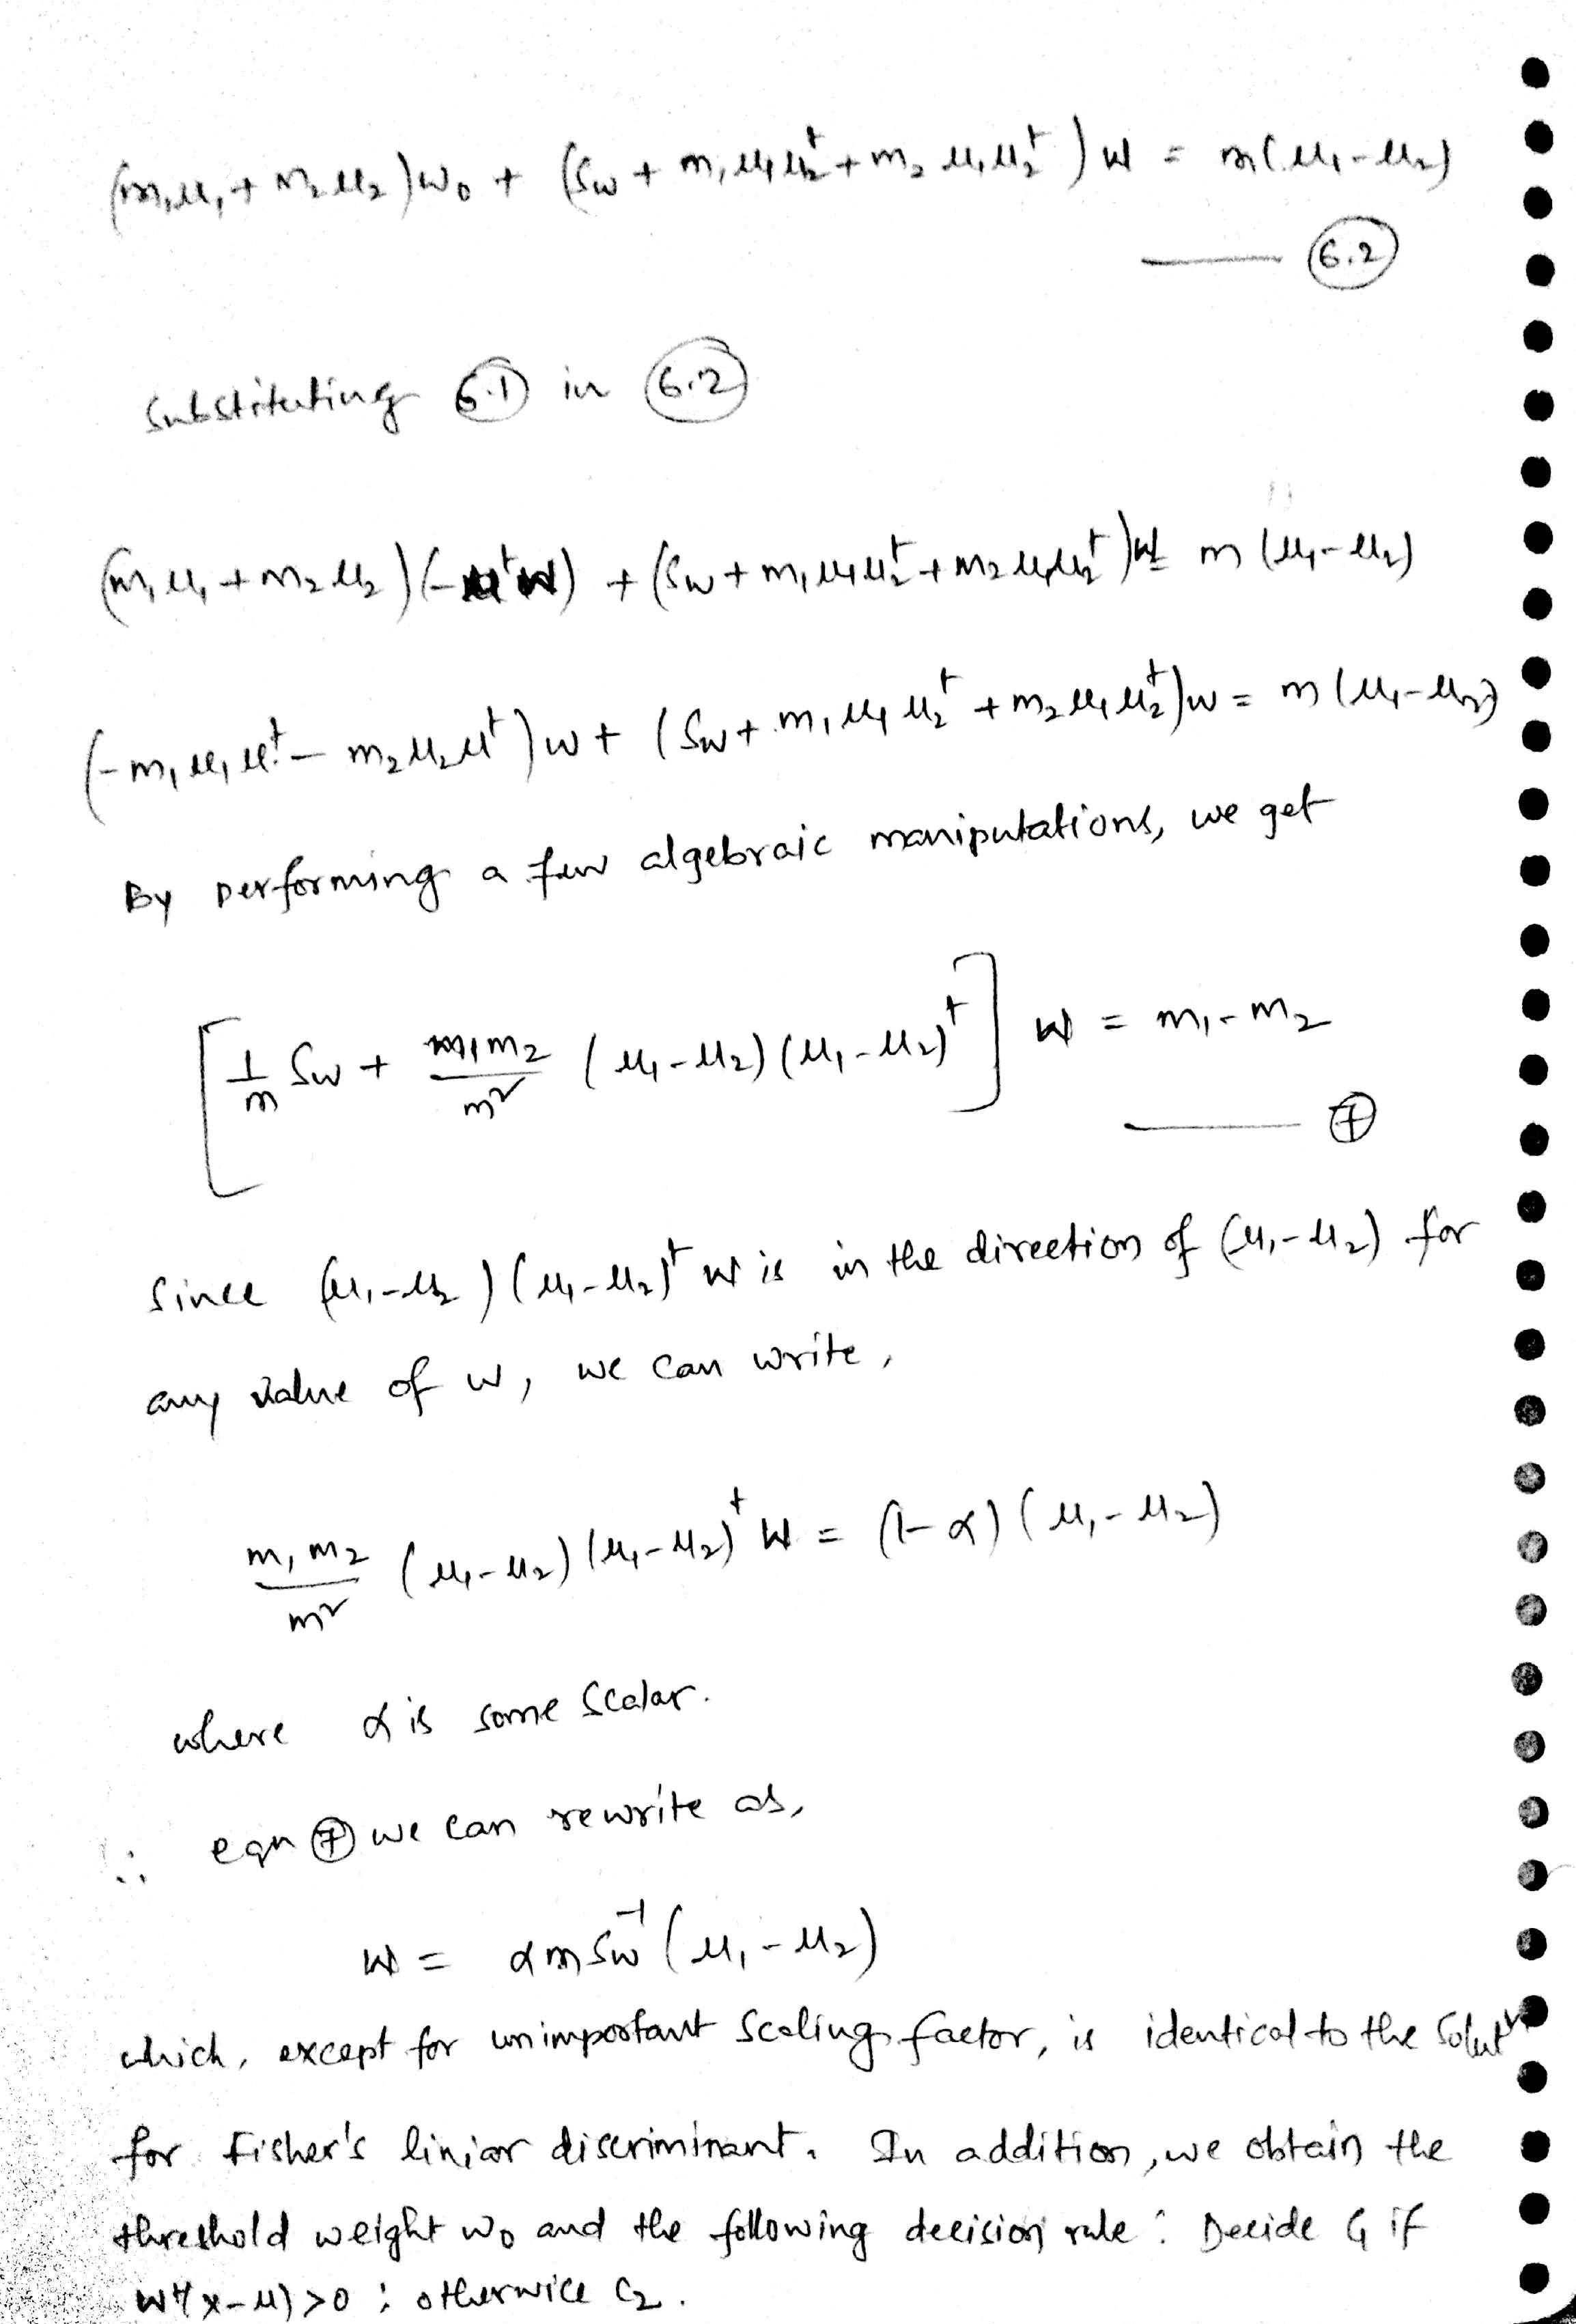
\includegraphics[scale=0.03]{images/p4A2_4.jpg}	
  \caption{p4}
  \label{fig:C34T2}
\end{figure}
\end{document}